\documentclass[a4paper,10pt,twoside]{book}

\usepackage{geometry}
\geometry{top=3cm,bottom=4cm}

\usepackage{ucs}
\usepackage[utf8x]{inputenc}
\usepackage[francais]{babel}
\usepackage[T1]{fontenc}
\usepackage{tabulary}

\usepackage[pdftex]{graphicx}
\usepackage[pdftex]{hyperref}
\hypersetup{%
   a4paper,
   bookmarksnumbered,
   bookmarksopen=true,
   bookmarksopenlevel=0,
   plainpages=false,
   unicode=true,
   colorlinks=true, 
   linkcolor=blue,
   urlcolor=blue,
   pdftitle={Manuel de l'utilisateur},
   pdfsubject={Manuel d'utilisation du logiciel XINX, editeur de feuille de style},
   pdfauthor={Ulrich Van Den Hekke}
}
\usepackage{nameref}
\usepackage{graphicx}
\usepackage{fancybox}
\usepackage{fancyvrb}
\usepackage{alltt}
\usepackage{color}

\author{Ulrich Van Den Hekke}
\date{05/05/2011}
\title{Manuel de l'utilisateur}

\begin{document}
  
\maketitle

\tableofcontents \addcontentsline{toc}{chapter}{Table des matières}

\chapter{Introduction}

XINX est un logiciel de développement essentielement tournée vers l'édition de feuille de style XSL, utilisé pour générer des fichiers HTML. 
Une feuille de style XSL est un fichier qui décrit une liste de transformation à appliquer à chaque noeud d'un fichier XML pour le transformer en un autre fichier text (Text plat, HTML, ou un autre fichier XML). Le domaine de XINX s'est un peu étendue dans l'édition des JavaScript et des feuilles de styles CSS associé à la page XSL.

Bref XINX est fait pour vous aider à développer votre site internet à base de feuille de style XSL.

\begin{center}
 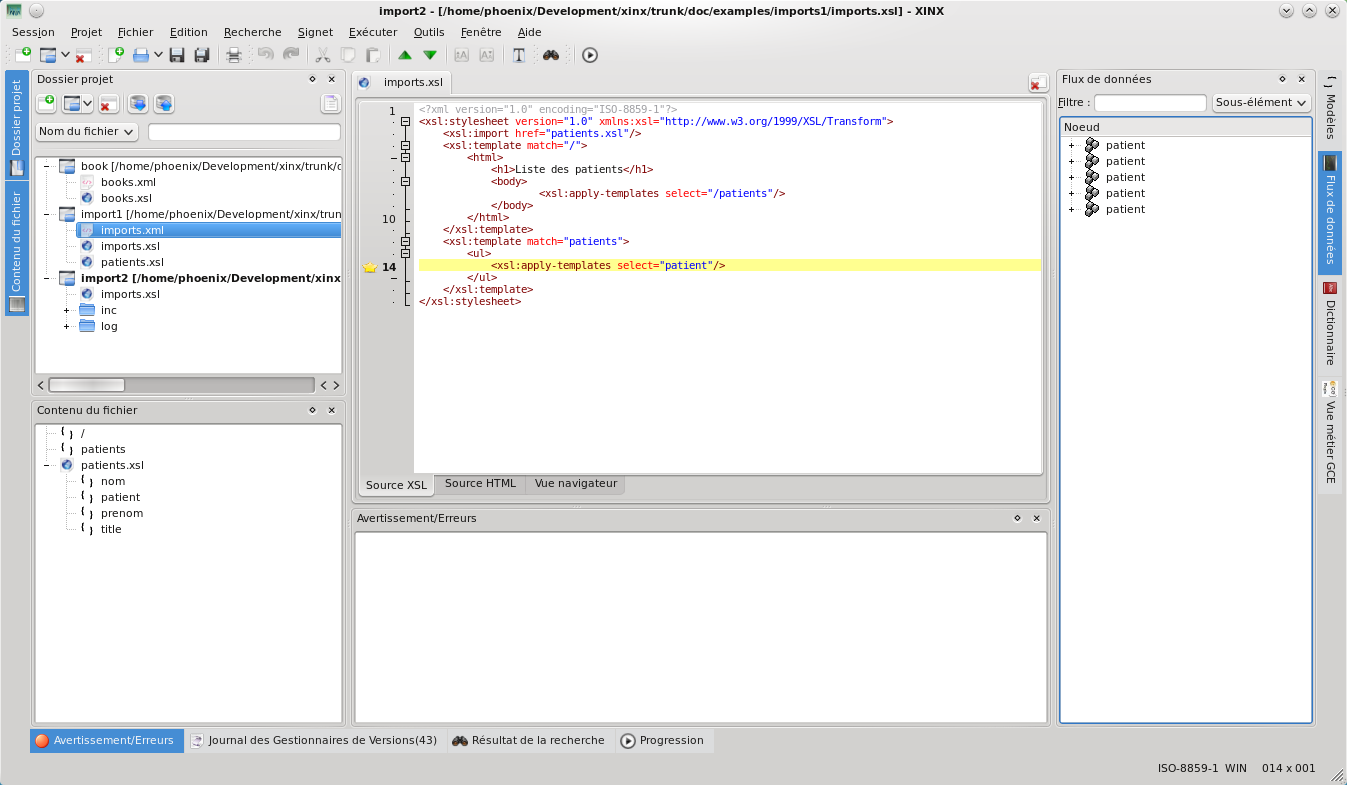
\includegraphics[width=\textwidth]{./mainform.png}
\end{center}

Le logiciel a été écris au début pour le développement des feuilles de styles de la société \href{http://www.generixgroup.com/}{Generix Group} et été fortement tournée vers cette technologie. Maintenant XINX se concentre sur le développement de feuille de style, et tout spécificité lié à la société Generix Group a été déporté dans un plugins. Vous pouvez donc maintenant utiliser XINX pour tout développement de feuille de style XSL.

Le logiciel XINX peut voir ses fonctionnalité étendue à l'aide de modèle (parfois aussi appelé snipet ou template), à l'aide de script (au format ECMAScript, proche de ce qu'est le JavaScript), ou à l'aide de plugins (écrit en C++ et en utilisant le framework Qt). Sinon XINX étant un logiciel libre il vous est toujours possible de faire évoluer le logiciel dans son intégralité, voir même de proposer un patch si c'est un besoin qui manque au logiciel.

XINX utilise le framework \href{http://qt.nokia.com}{Qt} comme base. Ce même framework est utilisé pour développé l'environnement de bureau \href{htpp://ww.kde.org}{KDE}, mais aussi des logiciels connues comme Skype, \ldots. Qt est n'est pas seulement un framework graphique mais propose quelques extentions au langauge C++ à l'aide des signaux, des slots, des pointeurs partagées, des listes, des boucles foreach, \ldots.

Ce manuel à pour but de vous aider à utiliser le logiciel XINX au mieux. Il vous expliquera comment installer le logiciel sur votre ordinateur, comment le paramètrer, puis comme l'utiliser pour développer vos feuilles de style.

\section{Utilisation des feuilles de style}

Les feuilles de styles XSL sont utilisé pour transformer un fichier XML en n'importe quel fichier text (plat, XML, HTML, ...). Vous pouvez ainsi transformer un même fichier XML en HTML, en tableau Excel, et en un fichier de donnée pour un WebServices à l'aide de plusieurs feuille de style.

Vous pouvez donc utiliser les feuilles XSL pour des transformation ponctuelles ou aussi pour des applications qui se base entièrement sur des feuilles XSL pour l'a présentation des données à l'utilisateur.

XSL signifie \emph{eXtensive Stylesheet Langage}, ou langage extensible de feuille de style. Quand on utilise des feuilles de styles, on utilise généralement deux technologies : 

\begin{itemize}
 \item \verb+XSLT+ est le language qui permet de transformer une arborescence de noeud d'un fichier XML donnée en un autre fichier de type texte (HTML, XML, texte, \dots.).
 \item \verb+XPath+ est la technologie utilisé pour accéder à n'importe quel noeud du fichier XML à l'aide d'un simple chemin. Les chemins sont écrit de la même manière que les chemins écrit pour accéder à un chemin sur le disque. Utilisation de \verb+/+ pour séparer les différents niveau. Différentes méthodes permette de compter un nombre de noeud.
\end{itemize}

Une feuille de style XSLT peut être utilisé pour filtrer un fichier XML, transformer le fichier en un autre fichier XML, générer une page HTML à partir d'un flux de donnée en XML. Un fichier de transformation XSL est lui même un fichier XML et doit donc respecter la norme XML elle même. Un éditeur de feuille de style XSL permet de faciliter l'édition des fichiers XML.

\section{Terminologie}

\section{Les fonctionnalités}

\subsection{Les types de fichiers}

XINX est un logiciel fort complet qui permet d'éditer principalement les feuilles de style mais permet également d'éditer d'autres type de fichiers.

XINX permet d'éditer les types de fichiers suivants:
\begin{itemsize}
  \item \verb+XSL Stylesheet+ : Le type de fichier que XINX sait le mieux éditer. Il propose une coloration syntaxique sur ce type de fichier, de l'autocompletion sur les balises, les attributs et sur les variables du fichier et sur les variables des fichiers d'import.
  \item \verb+XML File+ : La completion sur les fichiers XML n'existe pas, les balises des fichiers XML ne pouvant pas être déterminé à l'avance (sauf à part par un schema ou une DTD, mais XINX n'est pas encore capable de les utiliser). 
  \item \verb+HTML File+ : XINX est capable de compléter sur les fichiers HTML. Il propose les différentes balises HTML disponibles et les attributs associés. Pour certain attribut (comme l'attribut \verb+type+ de la balise \verb+input+), XINX propose aussi des valeurs.
  \item \verb+JavaScript+ : La coloration syntaxique est active sur ces fichiers. XINX est capable de faire de la completion basique sur les fichiers JavaScript. Certain fichiers JavaScript (utilisant la notion de prototype) ne sont pour l'instant pas lisible.
  \item \verb+Cascading Style Sheet+ : Seul la coloration syntaxique existe sur ce type de fichier. XINX est capable de vous présenter le contennu dans une boite à outil.
  \item \verb+XQuery+ : XINX est capable de proposer de la coloration syntaxique, ainsi que la completion sur quelques fonctions (count, \dots)
  \item \verb+Text file+ : Sur les fichiers textes, il n'y a pas de coloration syntaxique, ni de completion.
\end{itemsize}

Vous allez donc pouvoir développer dans un seul éditeur l'ensemble de vos feuilles de styles XSL ainsi que tous les autres fichiers associés à vos feuilles de styles\footnote{Si le besoin se fait sentir, vous pouvez développer un plugin pour gérer les autres types de fichiers associés à vos projets}.

\subsection{Le mode projet}

XINX possède un mode projet permettant de rassembler dans une seule vue l'enssemble des fichiers géré par XINX de votre projet. Cette vue vous permet alors de rechercher un fichier donnée de votre projet (pratique si votre projet possède beaucoup de fichier). Vous pouvez également ouvrir plusieurs projet en même temps. XINX fonctionne également sans utiliser sans le mode projet mais le mode projet permet d'accéder à des fonctionnalités supplémentaire et permet d'améliorer les propositons lors de la complétion.

\subsection{Les modèles}

Les modèles permettent d'améliorer la completion en faisant des propositions propre à votre utilisation, et propre à votre type de code. Les modèles sont des bouts de code qui sont ajouter automatiquement au votre quand vous écrivez un mot clé que vous avez choisit. Ce mot vous est proposé par la complétion de XINX.

Ces modèles sont utilisable par n'importe quel type de fichier.

\subsection{Les fichiers de données}

Une vue spéciale permet de visualiser les fichiers de données au format XML sous forme arborescente. Cette vue couplet avec une feuille de style ouverte permet également de tester votre feuille de style et d'en voir le résultat.

\chapter{Installation de XINX}

XINX possède différents paquets pour installer suivant l'environnement. Si vous avez déjà installé un logiciel auparavent sur votre système d'exploitation, l'installation vous sera facile. Comme l'installation du logiciel peut varier suivant la platforme, les instructions seront séparés dans plusieurs chapitre.

\section{MS/Windows}

Vous pouvez obtenir la version binaire de XINX pour les systèmes d'exploitations Ms/Windows sur la page de téléchargement du site de XINX à l'adresse \url{http://xinx.shadoware.org/wiki/Download}. 

Le démarrage de l'installation se fait par un double-clique sur le fichier executable de l'installation (nommé \verb+xinx-0.10.1.2531.exe+). Le programme install une version 32-bit de XINX. Il n'existe pas de version 64-bit de XINX.

Le programme vous demandera alors, après l'écran d'accueil, les composants que vous souhaiter installer avec XINX. Voici la liste des composants disponible :

\paragraph{Application et Bibliothèques necessaires} Ce paquet ne peux être déselectionner, il contient l'application et l'ensemble des bibliothèques necessaires à son fonctionnement.
\paragraph{Source de l'application} Ce paquet contient les sources de l'application que vous pouvez utiliser pour consultation, ou pour contribuer. Ce sont les sources qui ont été utilisé pour créer la version que vous installez. Les sources peuvent également être retrouvé sur le referenciel SubVersion. Vous n'êtez pas obligé d'installer ce paquet si vous n'avez pas l'intention de regarder les sources de l'application.
\paragraph{APIs de XINX} Ce paquet contient la documentation technique des différentes classes de XINX. Vous pouvez installer ce paquet si vous souhaiter apporter des modifications à XINX ou développer vos propre plugins.
\paragraph{Mode de fonctionnement Generix} Ce paquet permet d'installer le plugin qui vous permettra d'ajouter les fonctionnalités qui vous seront utils si vous développez des feuilles de style pour l'applicatif GCE. Pour plus d'information vous pouvez vous rendre à la section \ref{sec:Generix}.
\paragraph{Encapsulation de CVS} Ce plugin vous permet de coupler votre projet XINX avec le référenciel CVS. Pour plus d'information vous pouvez rendre à la section \ref{sec:RCS}. Il est necessaire d'avoir installer CVSNT pour pouvoir utiliser ce plugin.
\paragraph{Encapsulation de SubVersion} Ce plugin vous permet de coupler votre projet XINX avec le référenciel SubVersion. Pour plus d'information vous pouvez vous rendre à la section \ref{sec:RCS}. Il est necessaire d'avoir un client SubVersion d'installer (commande \verb+svn.exe+).
\paragraph{Plugin SubVersion pour XINX} Ce plugin vous permet de coupler votre projet XINX avec un référenciel SubVersion. Pour plus d'information vous pouvez vous rendre à la section \ref{sec:RCS}. Ce plugin ne necessite aucune dépendance. Vous pouvez alors utiliser SubVersion directement.
\paragraph{Appel de WebServices de type RPC} Ce plugin vous permet d'appeler des Services Internet de type RPC directement depuis XINX. Pour plus d'information vous pouvez vous rendre à la section \ref{sec:Services}.
\paragraph{Quelques scriptes} Ce paquet contient quelques scriptes utilitaire pouvant être appelé depuis XINX. Ces scripts sont écris dans un language proche du JavaScript. Voir la section \ref{sec:Scripts}.

Le programme d'installation créera un group XINX dans le menu <<Démaré>> de Windows qui vous permettra de lancer l'application et d'accéder à la documentation. Il vous sera également possible d'associer les fichier d'extentions \verb+.xsl+, \verb+.js+, et \verb+.fws+ avec XINX pour ouvrir automatiquement ce dernier lors du double clique sur un fichier portant l'une de ces extentions.

\section{Gnu/Linux}

\subsection{Version binaire pour Gnu/Debian}

Une version binaire de XINX est disponible pour la distribution Gnu/Debian. Vous pouvez la télécharger en ajoutant le dépôt \verb+http://apt.shadoware.org/+ à votre fichier \verb+/etc/apt/sources.list+ puis executant la commande d'installation de XINX. Votre gestionnaire de paquet s'occupera alors d'installer automatiquement les paquets manquants. 

XINX pour fonctionner necessite Qt, et les librairies libxml2 et libxslt1 de gestion des fichiers XML.

\begin{verbatim}
# echo "deb http://apt.shadoware.org/ squeeze main" >> /etc/apt/sources.list
# aptitude install xinx
\end{verbatim}

Vous pouvez alors démarrer XINX depuis le menu ou en le lancement depuis la ligne de commande. 

\subsection{Version source pour les autres distribution}

\paragraph{Récupérer les sources :}

Pour les autres distribution Gnu/Linux, il n'y a pas de paquet de disponible actuellement, il est néanmoins très facile de compiler XINX à partir des sources. Vous pouvez récupérer les sources de XINX sur la page de téléchargement à l'adresse \url{http://xinx.shadoware.org/wiki/Download}. Le fichier se présentera sous forme d'une archive \verb+.7z+. Vouz pourrez décompresser l'archive à l'aide de la commande :

\begin{verbatim}
# mkdir xinx
# cd xinx
# 7z x ../xinx-0.10.1.2531.7z
\end{verbatim}

\paragraph{Compilation :}

Sous Gnu/Linux la compilation necessite l'installation des paquets suivants\footnote{les paquets sont à titre d'exemple, il faudra adapter la liste des paquets enfonction de votre distribution.} :
\begin{itemize}
 \item libxml2-dev
 \item libxslt1-dev
 \item cmake
 \item libqt4-dev
 \item libsvncpp-dev 
\end{itemize}

Placer vous ensuite dans le dossier parent au dossier xinx et lancer la compilation à l'aide des commandes suivante :
\begin{verbatim}
# mkdir xinx-build
# cd xinx-build
# cmake ../xinx
# make
# sudo make install
\end{verbatim}

Si tout les paquets sont disponible la compilation et l'installation se passeront sans problème. En cas d'erreur, corrigé les paquets manquant et recommncer depuis le début.

\chapter{Interface principale de XINX}

Après l'installation, vous pouvez démarrer XINX comme suite :
\begin{itemize}
 \item Sous Windows, dans le menu << Démarrer >>, cliquez sur le programme dans le groupe XINX. Sous Vista et supérieur, vous pouvez aussi écrire directement <<XINX>> dans la boite de recherche du menu << Démarer >>
 \item Sous Linux, selon votre bureau, vous retrouver le programme XINX dans le groupe <<Developpement>> de votre menu d'application. Vous pouvez également tapper XINX dans le lanceur rapide ou dans une console Linux. 
\end{itemize}

Quand vous démarrez XINX pour la première fois, une fenêtre de configuration devrait s'ouvrir :

\begin{center}
 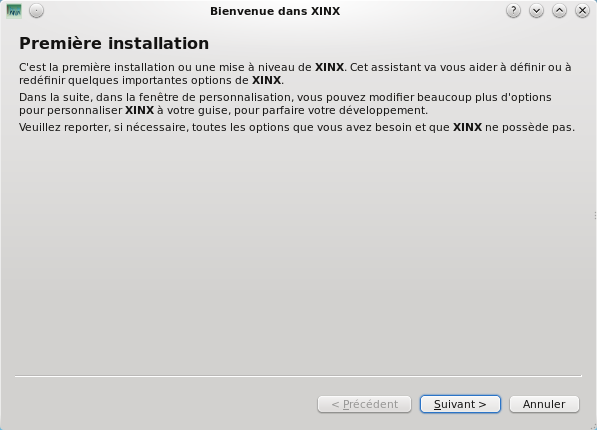
\includegraphics[width=0.60\textwidth]{./firstinstall1.png}
\end{center}

Cette fenêtre vous permettra de configurer les principales fonctionnalités de XINX. 

\begin{center}
 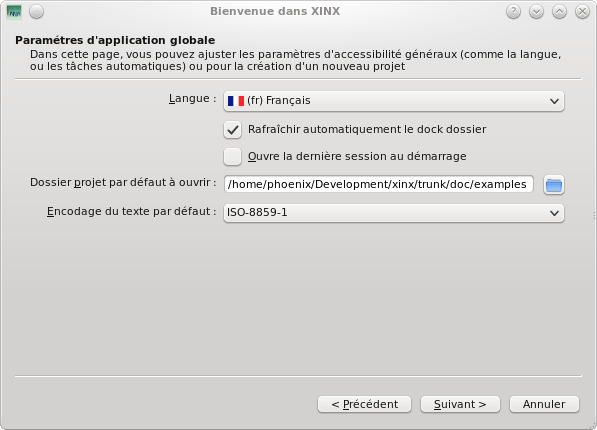
\includegraphics[width=0.60\textwidth]{./firstinstall2.png}
\end{center}

\paragraph{Langue} Sur la première page vous allez pouvoir choisir la langue d'affichage de XINX. 

\paragraph{Rafraichir automatiquement le dock dossier} Si vous décochez cette case, lorsque vous rechercherez un fichier dans un projet, il vous faudra frapper la touche <<Entrer>> pour lancer la recherche, sinon elle se lancera automatiquement à la fin de la frappe.

\paragraph{Ouvrir la dernière session au démarrage} Vous pouvez également indiquer que XINX doit ouvrir la dernière session au démarrage, avec les derniers projets ouvert. Si vous ne souhaiter pas ouvrir la dernière session au démarrage, XINX vous proposera dans une boîte de dialogue la liste des sessions disponible ainsi que la liste des projets possible.

\paragraph{Dossier projet à ouvrir par défaut} Le <<Dossier projet à ouvrir par défaut>> est le dossier qui vous sera proposé lorsque que vous allez créer un nouveau projet. C'est généralement le dossier qui se trouve au dessus de tous les dossiers sur lesquels vous allez travailler.

\paragraph{Encodage du texte par défaut} est l'encodage par défaut à utiliser pour les fichier dont XINX ne peux déterminer l'encodage (fichier texte, fichier JavaScript, \dots). Cette option n'a aucune effet sur les fichiers XML définissant au début du fichier l'encodage à utiliser.

\begin{center}
 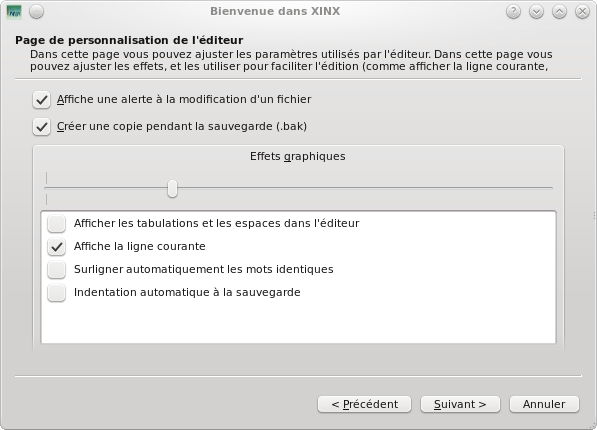
\includegraphics[width=0.60\textwidth]{./firstinstall3.png}
\end{center}

Sur l'écran suivant vous allez trouver différentes options lié à l'édition du texte. Si vous êtes familier avec d'autres IDE, vous reconnaitrez des options. 

\paragraph{Afficher une alerte à la modification d'un fichier} Lorsqu'un programme externe modifie un fichier ouvert dans XINX, ce dernier vous demandera alors automatiquement de recharger le fichier. Vous pourrez choisir de rafraichir ou non le document.

\paragraph{Créer une copie pendant la sauvegarde (.bak)} Lors de la sauvegarde, XINX peut créer pour vous un fichier \verb+.bak+ contenant la dernière version du fichier (avant sauvegarde). Vous pouvez ainsi retrouver une sauvegarde ancienne si nécessaire.

\paragraph{Afficher les tabulations et les espaces dans l'éditeur} Afficher les tabulations et les espaces dans l'éditeur de texte à l'aide d'un symbole pour mieux différencier les espaces et les tabulations.

\paragraph{Surligner automatiquement les mots identiques} Lorsque vous vous déplacer dans l'éditeur de texte, XINX surlignera tous les mots identiques au mot sous le curseur. A chaque déplacement, le surlignement sera mis à jours. Ceci peut avoir un impact sur les performances de XINX.

\paragraph{Indentation automatique à la sauvegarde} Lors de la sauvegarde, XINX réindentera automatiquement le document, si XINX est capable de gérer l'indentation de ce document. Actuellement seul les documents XML, XSLT, \dots et dérivés peuvent être indenté.

\begin{center}
 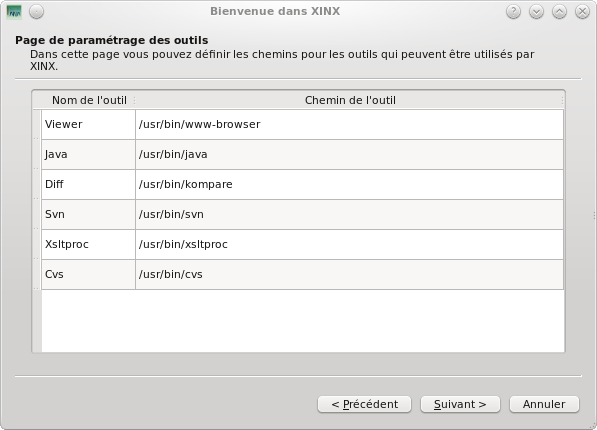
\includegraphics[width=0.60\textwidth]{./firstinstall4.png}
\end{center}

Enfin XINX vous demandera de définir l'emplacement d'une liste d'outil qu'il pourrait potentiellement avoir besoin. Si les outils ne sont pas installé, ou tout simplement, si vous ne souhaiter renseigner tout de suite ces outils, vous pouvez continuer. XINX vous re-demandera automatiquement l'outil lorsqu'il en aura besoin.

\section{L'interface principale}

L'interface principale de XINX est celle qui permet l'édition des fichiers. Elle propose différentes boîtes à outils offrant de l'aide à l'édition de XINX. Au centre de l'interface, se trouve la zone d'édition. Des onglets permette de choisir parmis les différents fichiers ouvert, celui que l'on souhaiter éditer.



\section{Les projets}

\section{Configuration de XINX}

\subsection{Création d'un projet}

\subsection{Utilisation des projets}
\label{sec:RCS}
Gestionnaire de version

\section{Mode édition}

\subsection{Edition}

\subsection{Test}

Flux de donnée / présentation

\section{Les onglets}

\chapter{Les modèles}

\chapter{Les scriptes}
\label{sec:Scripts}

\chapter{Les extentions}

\section{Services}
\label{sec:Services}


Type de fichier : Web Service Stream


\section{Generix}
\label{sec:Generix}

Type de fichier : Generix Maquette File.

\appendix
\chapter{Les raccourcis}

\chapter{Interface ECMAScript de XINX}

\chapter{Point de vue technique}

\section{Où sont stocker les fichiers de XINX}

\chapter{Dépannage}

\chapter{Limitations connues}

\chapter{Logiciels tiers et licence}

\chapter{Glossaire}

\end{document}
